% !TeX spellcheck = cs_CZ
%{\tikzset{external/prefix={tikz/FYZII/}}
% \tikzset{external/figure name/.add={ch38_}{}}
%---------------------------------------------------------------------------------------------------
% file fey2ch38.tex
%---------------------------------------------------------------------------------------------------
%=========================== Kapitola Pružnost =====================================================
\setchaptertoc
\chapter{Pružnost}\label{fyz:IIchapIIXL}

  \section{Hookeův zákon}\label{fyz:IIchapIIXLsecI}
  \section{Homogenní deformace}\label{fyz:IIchapIIXLsecII}
  \section{Torzní tyč. Střižné vlny}\label{fyz:IIchapIIXLsecIII}
  \section{Prohnutý nosník}\label{fyz:IIchapIIXLsecIV}
  \section{Vzpěrnost}\label{fyz:IIchapIIXLsecV}
  \section{Příklady a cvičení}\label{fyz:IIchapIIXLsecVI}
  

    \begin{figure}[ht!] %\ref{fyz:fig0799}
      \centering
      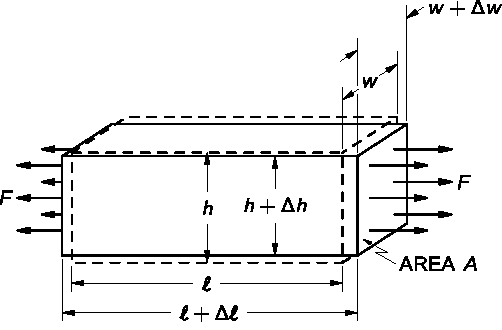
\includegraphics[width=0.7\linewidth]{fyz_fig0799.pdf}
      \caption{
               (\cite[s.~707]{Feynman02})}
      \label{fyz:fig0799}
    \end{figure}
    
    \begin{figure}[ht!] %\ref{fyz:fig0800}
      \centering
      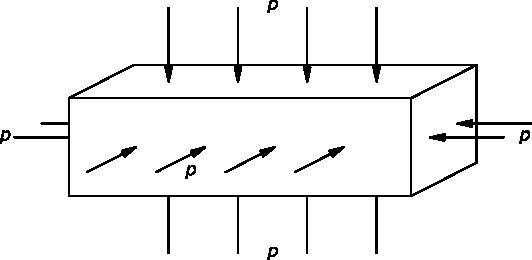
\includegraphics[width=0.7\linewidth]{fyz_fig0800.pdf}
      \caption{
               (\cite[s.~707]{Feynman02})}
      \label{fyz:fig0800}
    \end{figure}

    \begin{figure}[ht!]
      \centering
      \subcaptionbox{\label{fyz:fig0801a}}{\luafigure[0.9]{fyz_fig0801a.pdf}}               \\
      \subcaptionbox{\label{fyz:fig0801b}}{\luafigure[0.9]{fyz_fig0801b.pdf}}               \\
      \subcaptionbox{\label{fyz:fig0801c}}{\luafigure[0.9]{fyz_fig0801c.pdf}}
      \caption{
               (\cite[s.~748]{Feynman02})}
      \label{fyz:fig0801}
    \end{figure}

    \begin{figure}[ht!] %\ref{fyz:fig0802}
      \centering
      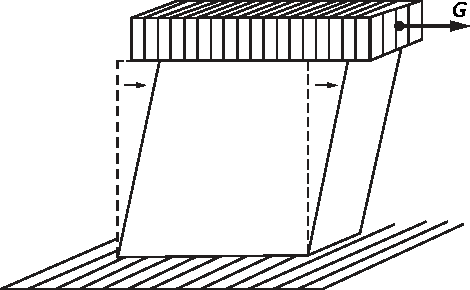
\includegraphics[width=0.7\linewidth]{fyz_fig0802.pdf}
      \caption{
               (\cite[s.~707]{Feynman02})}
      \label{fyz:fig0802}
    \end{figure}
    
    \begin{figure}[ht!] %\ref{fyz:fig0803}
      \centering
      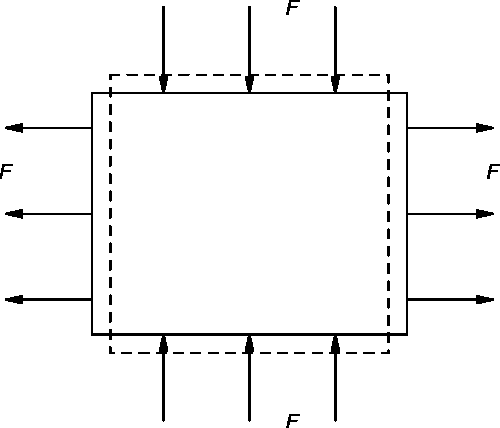
\includegraphics[width=0.7\linewidth]{fyz_fig0803.pdf}
      \caption{
               (\cite[s.~707]{Feynman02})}
      \label{fyz:fig0803}
    \end{figure}

    \begin{figure}[ht!] %\ref{fyz:fig0804}
      \centering
      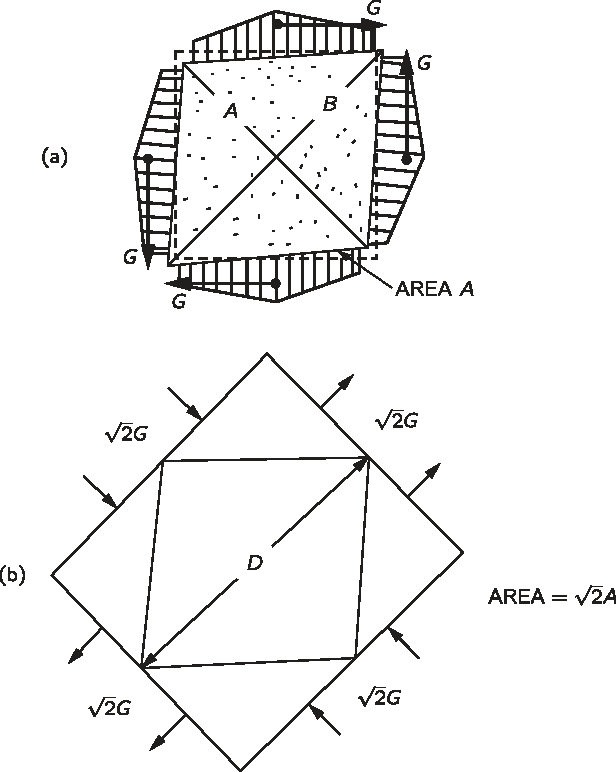
\includegraphics[width=0.7\linewidth]{fyz_fig0804.pdf}
      \caption{
               (\cite[s.~707]{Feynman02})}
      \label{fyz:fig0804}
    \end{figure}
    
    \begin{figure}[ht!] %\ref{fyz:fig0805}
      \centering
      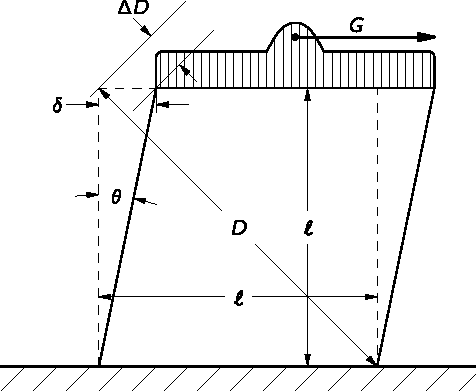
\includegraphics[width=0.7\linewidth]{fyz_fig0805.pdf}
      \caption{
               (\cite[s.~707]{Feynman02})}
      \label{fyz:fig0805}
    \end{figure}


    \begin{figure}[ht!] %\ref{fyz:fig0806}
      \centering
      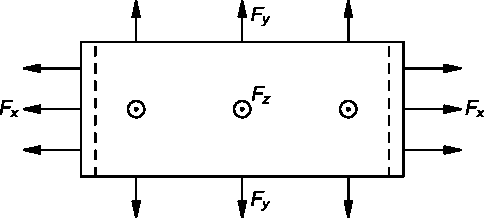
\includegraphics[width=0.7\linewidth]{fyz_fig0806.pdf}
      \caption{
               (\cite[s.~707]{Feynman02})}
      \label{fyz:fig0806}
    \end{figure}

    \begin{figure}[ht!] %\ref{fyz:fig0807}
      \centering
      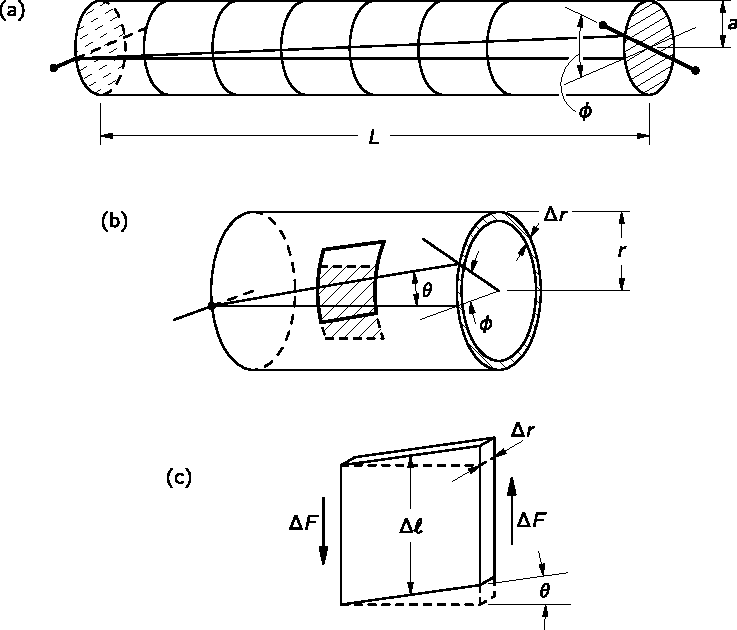
\includegraphics[width=0.7\linewidth]{fyz_fig0807.pdf}
      \caption{
               (\cite[s.~707]{Feynman02})}
      \label{fyz:fig0807}
    \end{figure}
    
    \begin{figure}[ht!] %\ref{fyz:fig0808}
      \centering
      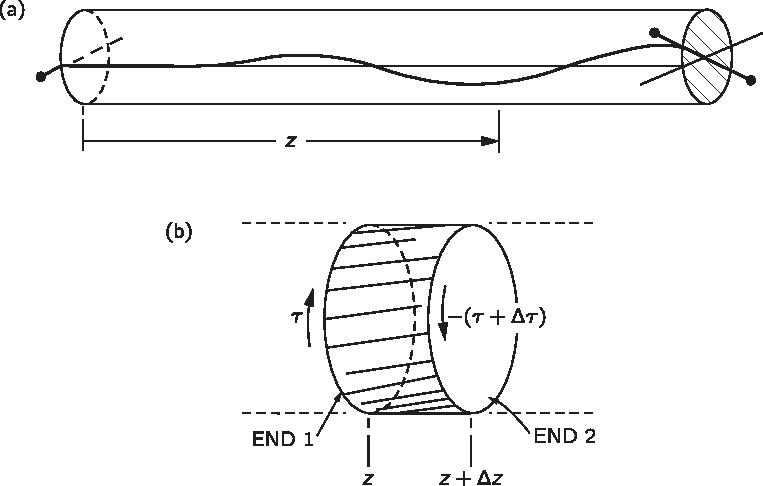
\includegraphics[width=0.7\linewidth]{fyz_fig0808.pdf}
      \caption{
               (\cite[s.~707]{Feynman02})}
      \label{fyz:fig0808}
    \end{figure}

    \begin{figure}[ht!] %\ref{fyz:fig0809}
      \centering
      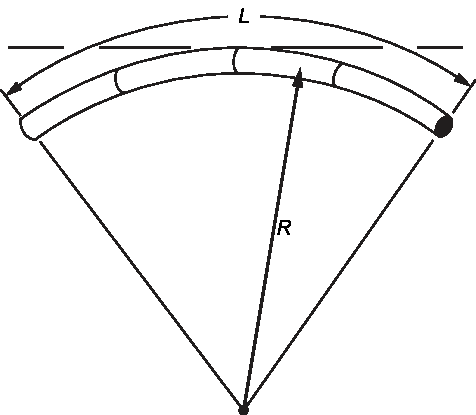
\includegraphics[width=0.7\linewidth]{fyz_fig0809.pdf}
      \caption{
               (\cite[s.~707]{Feynman02})}
      \label{fyz:fig0809}
    \end{figure}
    
    \begin{figure}[ht!] %\ref{fyz:fig0810}
      \centering
      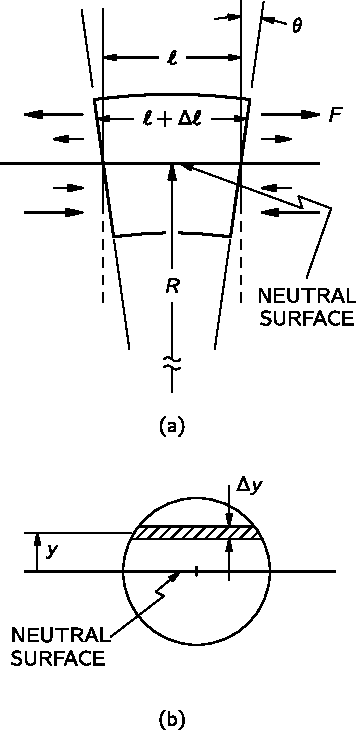
\includegraphics[width=0.7\linewidth]{fyz_fig0810.pdf}
      \caption{
               (\cite[s.~707]{Feynman02})}
      \label{fyz:fig0810}
    \end{figure}


    \begin{figure}[ht!] %\ref{fyz:fig0811}
      \centering
      
\includegraphics[width=0.7\linewidth]{fyz_fig0811.pdf}
      \caption{
               (\cite[s.~707]{Feynman02})}
      \label{fyz:fig0811}
    \end{figure}

    \begin{figure}[ht!] %\ref{fyz:fig0812}
      \centering
      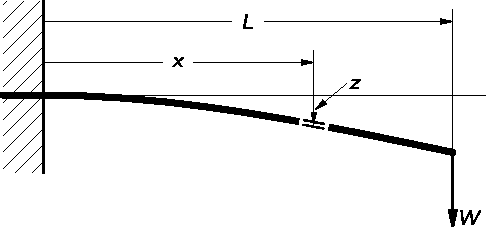
\includegraphics[width=0.7\linewidth]{fyz_fig0812.pdf}
      \caption{
               (\cite[s.~707]{Feynman02})}
      \label{fyz:fig0812}
    \end{figure}
    
    \begin{figure}[ht!] %\ref{fyz:fig0813}
      \centering
      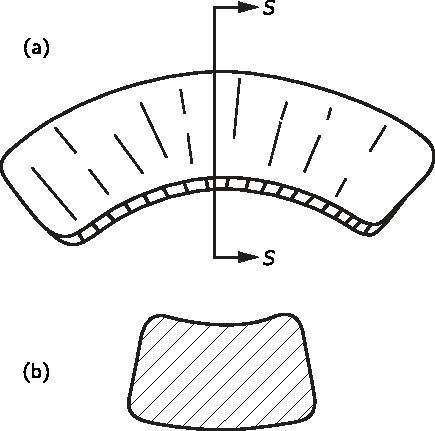
\includegraphics[width=0.7\linewidth]{fyz_fig0813.pdf}
      \caption{
               (\cite[s.~707]{Feynman02})}
      \label{fyz:fig0813}
    \end{figure}

    \begin{figure}[ht!] %\ref{fyz:fig0814}
      \centering
      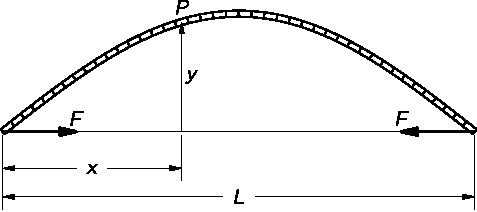
\includegraphics[width=0.7\linewidth]{fyz_fig0814.pdf}
      \caption{
               (\cite[s.~707]{Feynman02})}
      \label{fyz:fig0814}
    \end{figure}
    
    \begin{figure}[ht!] %\ref{fyz:fig0815}
      \centering
      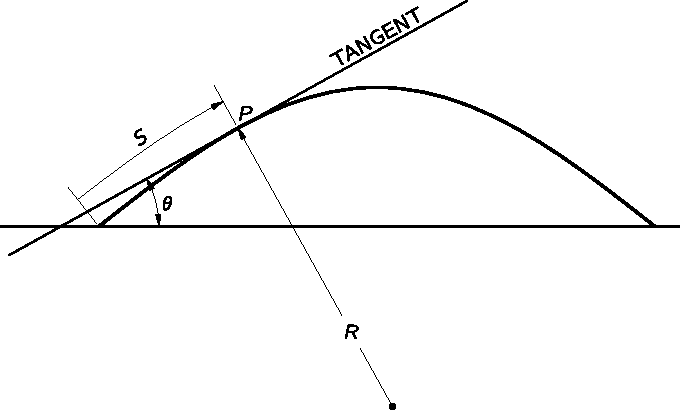
\includegraphics[width=0.7\linewidth]{fyz_fig0815.pdf}
      \caption{
               (\cite[s.~707]{Feynman02})}
      \label{fyz:fig0815}
    \end{figure}


    \begin{figure}[ht!] %\ref{fyz:fig0816}
      \centering
      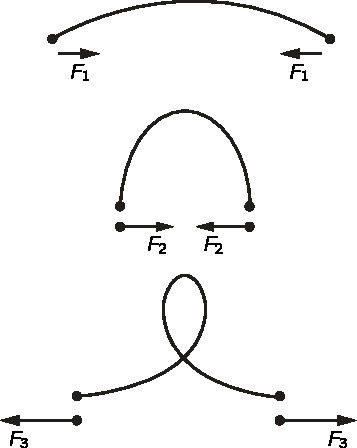
\includegraphics[width=0.7\linewidth]{fyz_fig0816.pdf}
      \caption{
               (\cite[s.~707]{Feynman02})}
      \label{fyz:fig0816}
    \end{figure}

    \todo[inline]{Kapitola fey2ch38 je nedodělaná, obsahuje pouze obrázky}

%} %tikzset
%---------------------------------------------------------------------------------------------------
